% ShareWood — diapos du pitch (Beamer, 16:9). Compiler : latexmk -pdf sharewood.tex (voir README.md).
%
% POUR MODIFIER : chaque diapo est un bloc « \begin{frame} ... \end{frame} » repéré par un titre en capitales.
% Les positions sont en « pixels » sur une diapo de 1920 x 1080 : (0,0) en haut à gauche, y vers le bas.
%   \txt{x}{y}{largeur}{taille}{couleur}{texte}   un texte posé à cet endroit
%   \card{x}{y}{largeur}{hauteur}{fond}           un rectangle arrondi
%   \phone{x}{y}{largeur}{image}                  une capture dans un cadre de téléphone
\documentclass[aspectratio=169]{beamer}

\usepackage[T1]{fontenc}
\usepackage[utf8]{inputenc}
\usepackage[french]{babel}
\frenchsetup{StandardLists=true}
\usepackage{inter}                   % texte courant
\usepackage{sourceserifpro}          % titres (chargé après : c'est lui la police « romaine »)
\renewcommand{\familydefault}{\sfdefault}
\usepackage{tikz}
\graphicspath{{images/}}

% --- Notes d'orateur : retirer le « % » pour les afficher à droite de chaque diapo ---
% \setbeameroption{show notes on second screen=right}

% --- Couleurs de l'application ---
\definecolor{paper}{HTML}{F1EFE9}
\definecolor{surface}{HTML}{FAF9F5}
\definecolor{border}{HTML}{DDD9CF}
\definecolor{ink}{HTML}{1A1A18}
\definecolor{muted}{HTML}{55544F}
\definecolor{forest}{HTML}{1E3A2F}
\definecolor{forestdark}{HTML}{10241C}
\definecolor{plum}{HTML}{4B2A63}
\definecolor{night}{HTML}{1D1029}
\definecolor{sage}{HTML}{CFE3CA}
\definecolor{gold}{HTML}{F2C14E}

\setbeamertemplate{navigation symbols}{}

% --- Outils de mise en page ---
\newlength{\pxu}
\setlength{\pxu}{0.0833333mm}        % 1 « pixel » : 160 mm / 1920
\newcommand{\size}[1]{\fontsize{\the\dimexpr#1\pxu\relax}{\the\dimexpr#1\pxu*128/100\relax}\selectfont}
\newcommand{\titre}{\rmfamily\bfseries}
\newcommand{\txt}[6]{\node[anchor=north west, inner sep=0pt, text width=#3\pxu, align=flush left, text=#5] at (#1,#2) {\size{#4}#6\par};}
\newcommand{\ctxt}[6]{\node[anchor=north, inner sep=0pt, text width=#3\pxu, align=center, text=#5] at (#1,#2) {\size{#4}#6\par};}
\newcommand{\card}[5]{\fill[#5, rounded corners=40\pxu] (#1,#2) rectangle +(#3,#4);}
% Capture de téléphone (proportions 780 x 1688) avec son cadre.
\newcommand{\phone}[4]{%
  \pgfmathsetmacro{\ph}{#3*2.16410}%
  \fill[black!92, rounded corners=48\pxu] (#1,#2) rectangle +({#3+24},{\ph+24});
  \begin{scope}
    \clip[rounded corners=36\pxu] ({#1+12},{#2+12}) rectangle +(#3,\ph);
    \node[anchor=north west, inner sep=0pt] at ({#1+12},{#2+12}) {\includegraphics[width=#3\pxu]{#4}};
  \end{scope}}
% Liste à puces compacte, utilisable dans un \txt.
\newcommand{\puce}[1]{\hangindent=1.1em\hangafter=1 \makebox[1.1em][l]{\textbullet}#1\par\vspace{0.35em}}
% Une diapo : \diapo{fond}{contenu tikz}
\newcommand{\diapo}[2]{%
  \begin{tikzpicture}[remember picture, overlay, shift={(current page.north west)}, x=\pxu, y=-\pxu]
    #1
    #2
  \end{tikzpicture}}
\newcommand{\fondclair}{\fill[paper] (0,0) rectangle (1920,1080);}
\newcommand{\fondvert}{\shade[top color=forest, bottom color=forestdark] (0,0) rectangle (1920,1080);}
\newcommand{\fondviolet}{\shade[top color=plum, bottom color=night] (0,0) rectangle (1920,1080);}

\begin{document}

% =============================== 1. INTRODUCTION ===============================
\begin{frame}[plain]
\diapo{\fondvert}{
  \node[anchor=north west, inner sep=0pt] at (96,66) {
\includegraphics[width=100\pxu]{logo}};
  \draw[sage, line width=3\pxu] (146,116) circle (50);
  \txt{224}{80}{360}{60}{surface}{\titre ShareWood}
  \txt{590}{100}{700}{36}{sage}{\rmfamily\itshape Les bons plans se partagent.}
  \node[anchor=north east, inner sep=0pt, text=sage] at (1824,102) {\size{30}Anne-Lise · Justin · Matteo · Sacha};
  % Le paradoxe : grand titre, puis deux colonnes face à face, et la conséquence en or.
  \txt{96}{215}{1728}{88}{surface}{\titre Hyperconnectés, mais \textcolor{gold}{mal informés.}}
  \txt{96}{340}{1728}{40}{sage}{\rmfamily\itshape C'est le paradoxe de notre génération.}
  \card{96}{470}{800}{280}{surface}
  \txt{146}{514}{700}{26}{plum}{\bfseries CE QUE NOUS SOMMES}
  \txt{146}{566}{700}{46}{forest}{\titre La génération la plus connectée de l'histoire.}
  \ctxt{960}{545}{128}{120}{gold}{\titre $\neq$}
  \card{1024}{470}{800}{280}{gold}
  \txt{1074}{514}{700}{26}{forestdark}{\bfseries CE QUI SE PASSE}
  \txt{1074}{566}{700}{46}{ink}{\titre Et pourtant, personne ne nous parle des bons plans.}
  \fill[sage] (900,820) rectangle +(120,4);
  \ctxt{960}{855}{1700}{52}{gold}{\rmfamily\itshape Rater un bon plan, c'est payer plus cher sans même le savoir.}
}
\note{Hyperconnectés, mais mal informés : c'est le paradoxe de notre génération. Nous sommes la plus connectée de l'histoire, et pourtant les bons plans étudiants circulent encore… de bouche à oreille. Le problème, c'est que pour un étudiant, chaque euro compte, et passer à côté d'un bon plan, c'est payer plus cher sans même le savoir. Les bons plans existent, mais ils restent cachés, éparpillés, réservés à ceux qui ont la bonne info au bon moment.}
\end{frame}

% =============================== 2. SOLUTION ===============================
\begin{frame}[plain]
\diapo{\fondclair}{
  \txt{96}{80}{1200}{26}{plum}{\bfseries NOTRE SOLUTION}
  \txt{96}{140}{1240}{92}{forest}{\titre ShareWood, fini le hasard}
  \txt{96}{290}{1180}{44}{ink}{Les bons plans étudiants au même endroit, partagés et vérifiés par la communauté.}
  \card{96}{460}{588}{270}{forest}
  \txt{136}{496}{510}{52}{surface}{\titre Trouver}
  \txt{136}{590}{510}{36}{surface}{Une carte et un fil «~Pour~toi~».}
  \card{716}{460}{588}{270}{plum}
  \txt{756}{496}{510}{52}{surface}{\titre Partager}
  \txt{756}{590}{510}{36}{surface}{Une photo, le formulaire se remplit.}
  \card{96}{762}{588}{270}{gold}
  \txt{136}{798}{510}{52}{ink}{\titre Vérifier}
  \txt{136}{892}{510}{36}{ink}{«~J'en ai profité~» ou «~Plus dispo~».}
  \card{716}{762}{588}{270}{surface}
  \txt{756}{798}{510}{52}{forest}{\titre Nettoyer}
  \txt{756}{892}{510}{36}{ink}{Trois signalements, et l'offre devient «~Douteux~».}
  \phone{1396}{74}{406}{carte}
}
\note{Nous avons créé ShareWood pour mettre fin à cette injustice. Les étudiants partagent les offres autour d'eux, et la communauté les vérifie : fini le hasard.}
\end{frame}

% =============================== 3. DÉMONSTRATION (vidéo promo : un clic ouvre pitch/sharewood-promo.mp4) ===============================
% Le MP4 doit rester à côté du PDF. Acrobat demande l'autorisation d'ouvrir le fichier au premier clic ;
% Aperçu (macOS) ne suit pas ce type de lien : ouvrir alors la vidéo à la main.
\begin{frame}[plain]
\diapo{\fondclair}{
  \ctxt{960}{60}{1728}{80}{forest}{\titre Comment ça marche, concrètement}
  % Téléphone (écran 484 × 860, proportions de la vidéo 1080 × 1920) avec la vidéo à 23 s
  \fill[black!92, rounded corners=48\pxu] (706,170) rectangle +(508,884);
  \begin{scope}
    \clip[rounded corners=36\pxu] (718,182) rectangle +(484,860);
    \node[anchor=north west, inner sep=0pt] at (718,182) {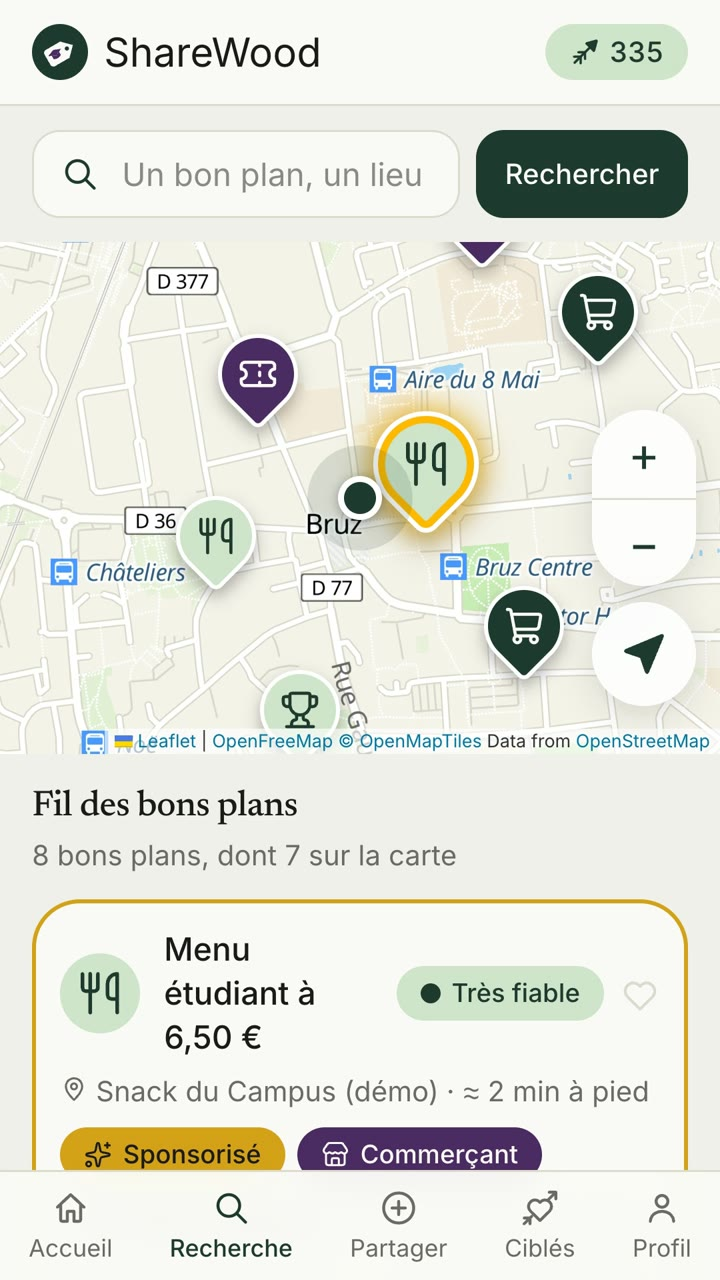
\includegraphics[width=484\pxu]{promo-affiche}};
  \end{scope}
  % Bouton lecture
  \fill[forest, opacity=0.88] (960,612) circle (78);
  \fill[surface] (936,568) -- (936,656) -- (1012,612) -- cycle;
  % Zone cliquable : tout le téléphone
  \node[anchor=north west, inner sep=0pt] at (706,170) {\href{run:sharewood-promo.mp4}{\rule{0pt}{884\pxu}\hspace{508\pxu}}};
}
\note{Je vous montre comment ça marche concrètement. (Cliquer sur le téléphone : la vidéo s'ouvre dans le lecteur vidéo ; Acrobat demande l'autorisation la première fois. La passer en plein écran, puis revenir au PDF. Elle dure 59 s, sans son.) On crée son profil en quelques gestes ; l'accueil et la carte montrent les bons plans autour de soi ; on cherche « piscine » et on confirme l'offre avec « J'en ai profité » ; on partage un bon plan en le prenant en photo ; et on retrouve ses Flèches et la boutique de récompenses.}
\end{frame}

% =============================== 4. TROIS PILIERS ===============================
\begin{frame}[plain]
\diapo{\fondclair}{
  \txt{96}{80}{1200}{26}{plum}{\bfseries NOS TROIS PILIERS}
  \txt{96}{140}{1728}{80}{forest}{\titre Ancré dans le réel, ouvert à tous, rapide}
  \card{96}{300}{555}{690}{forest}
  \txt{140}{350}{470}{52}{surface}{\titre 1 · Du réel}
  \txt{140}{460}{480}{44}{surface}{\puce{Manger et courses}\puce{Voyager}\puce{Aides et bourses}\puce{Sport et culture}}
  \card{683}{300}{555}{690}{plum}
  \txt{727}{350}{480}{52}{surface}{\titre 2 · Égalité d'accès}
  \txt{727}{460}{480}{44}{surface}{\puce{Gratuit}\puce{Ouvert à tous}\puce{Commerçants locaux visibles}}
  \card{1269}{300}{555}{690}{gold}
  \txt{1313}{350}{480}{52}{ink}{\titre 3 · Rapidité}
  \txt{1313}{460}{480}{44}{ink}{\puce{Une carte}\puce{Des filtres}\puce{Un geste pour valider}}
}
\note{ShareWood, c'est trois choses. Un ancrage dans le réel : aucune marque imposée, on s'adapte à vos pratiques et à tous les profils. L'égalité d'accès : le bon plan n'est plus réservé aux initiés, et les petits commerçants deviennent visibles. La rapidité : une carte, des filtres, un geste.}
\end{frame}

% =============================== 5. MODÈLE ÉCONOMIQUE ===============================
\begin{frame}[plain]
\diapo{\fondclair}{
  \txt{96}{80}{1200}{26}{plum}{\bfseries NOTRE MODÈLE}
  \txt{96}{140}{1728}{76}{forest}{\sffamily\bfseries ADAPTABILITÉ \textcolor{plum}{·} ÉGALITÉ \textcolor{plum}{·} FACILITÉ}
  \card{96}{300}{640}{210}{forest}
  \txt{136}{334}{560}{52}{surface}{\titre L'étudiant}
  \txt{136}{424}{580}{36}{surface}{Gratuit, avec des récompenses.}
  \card{96}{530}{640}{210}{surface}
  \txt{136}{564}{560}{52}{forest}{\titre Le commerçant}
  \txt{136}{654}{580}{36}{ink}{Ses offres et leurs résultats.}
  \card{96}{760}{640}{240}{gold}
  \txt{136}{794}{580}{52}{ink}{\titre Le temps}
  \txt{136}{884}{560}{36}{ink}{Rapidité et Facilité}
  \begin{scope}
    \clip[rounded corners=32\pxu] (768,300) rectangle (1824,960);
    \node[anchor=north west, inner sep=0pt] at (768,300) {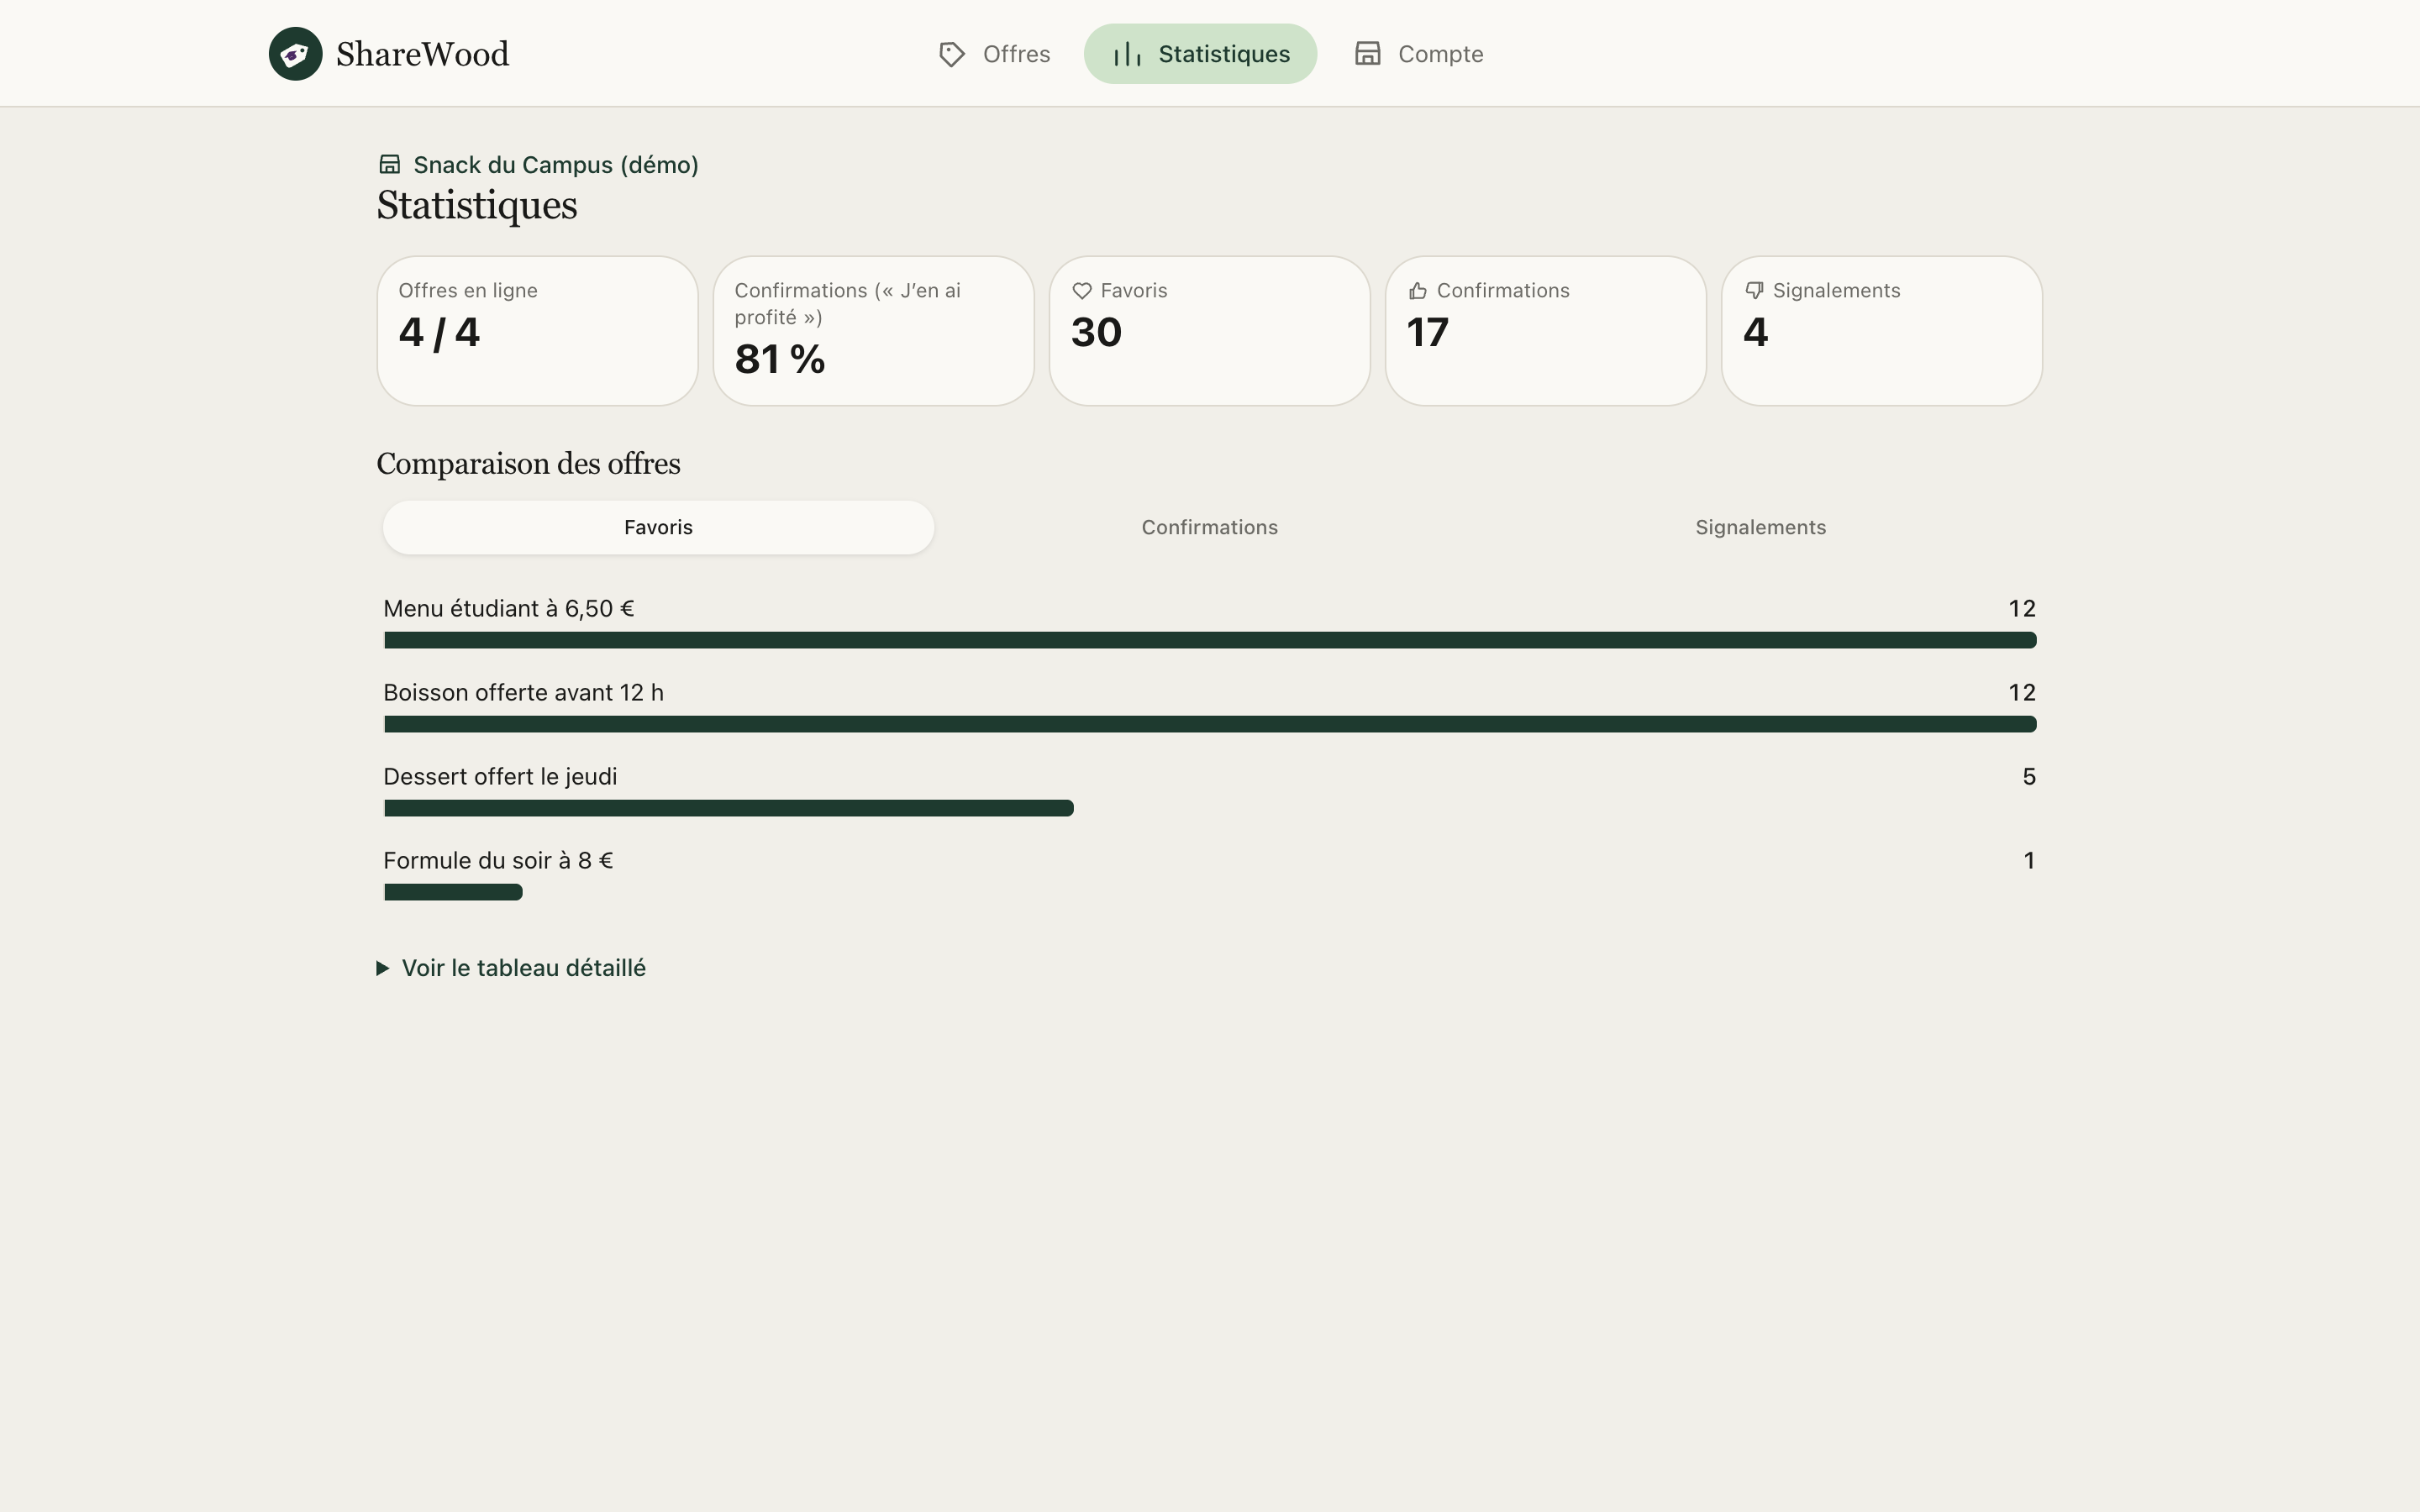
\includegraphics[width=1056\pxu]{statistiques}};
  \end{scope}
  \draw[forest, line width=3\pxu, rounded corners=32\pxu] (768,300) rectangle (1824,960);
}
\note{Pour les étudiants, c'est gratuit. Les commerçants, eux, peuvent payer pour mettre leur offre en avant, et suivre ses résultats.}
\end{frame}

% =============================== 6. CONCLUSION ===============================
\begin{frame}[plain]
\diapo{\fondvert}{
  \node[anchor=north, inner sep=0pt] at (960,62) {
\includegraphics[width=104\pxu]{logo}};
  \draw[sage, line width=4\pxu] (960,114) circle (52);
  \ctxt{960}{200}{1728}{80}{surface}{\titre Le bouche-à-oreille devient\\un \textcolor{gold}{réflexe collectif}}
  \card{96}{460}{555}{200}{surface}
  \txt{136}{494}{480}{52}{forest}{\titre Fini le hasard}
  \txt{136}{582}{480}{36}{ink}{Tout au même endroit.}
  \card{683}{460}{555}{200}{surface}
  \txt{723}{494}{480}{52}{forest}{\titre La confiance}
  \txt{723}{582}{480}{36}{ink}{Vérifié par les étudiants.}
  \card{1269}{460}{555}{200}{surface}
  \txt{1309}{494}{480}{52}{forest}{\titre Et demain}
  \txt{1309}{582}{480}{36}{ink}{Jusqu'en Erasmus.}
  \ctxt{960}{730}{1728}{72}{gold}{\rmfamily\itshape Merci ! Vos questions ?}
  \fill[surface, rounded corners=40\pxu] (610,880) rectangle (1310,960);
  \ctxt{960}{900}{700}{34}{forest}{\bfseries \href{https://sharewood-ensai.vercel.app}{sharewood-ensai.vercel.app}}
}
\note{ShareWood transforme le bouche-à-oreille en un réflexe collectif, simple et solidaire, pour redonner du pouvoir d'achat aux étudiants. Merci, nous attendons vos questions !}
\end{frame}

\end{document}

